\chapter{Counting}

The ``counting'' we address here in a discrete mathematical sense is not about counting from number to number in an arithmetic sequence. It's about estimating the number of possibilities. \\
Consider a deck of 40 cards. What is the probability from which you draw all 5 parts of the inexorable Exodia? What is the total number of cases about the combination of 5 cards you draw from your deck, and from there within, what are all possible cases of drawing five cards of some same category (number 8, club, diamond...)? \\
Most importantly, what is the probability of it? \\
The techniques we employ to estimate and learn the total number of possible cases according to some conditions is known as \textbf{counting}. \\
In this chapter, let us begin from counting in simpler circumstances, like counting sequences.

\section{Sampling without Replacement}
\subsection{Counting Sequences}
Let there be a set $S = \{1, 2, \cdots, n\}$. \\
We may pick $k \leq n$ elements from this set $S$, one at a time, while removing what we have sampled (selected) from $S$. This is known as \textbf{sampling without replacement}: once we select something from a set, it is removed from the set. \\
When counting the number of different ways to do this, either order matters, or order doesn't. In the case that order does matter, we are counting ordered sequences.

The most daily-life example would be Poker. \\
When we deal a card, that card dissappears is removed from the deck. The card is being sampled without replacement of it back into the card.
Meanwhile, when the sequence is ordered, the sequence of dealing card A then card B is different from the sequence of dealing card B then card A: in a sequence, order matters. \\
Therefore, at the first card, we have 52 disctinct possibilities for the card we now deal. \\
The second card, however, depends on the first card, since it cannot coincide with the first card. Your hand cannot have two exactly same card. That is cheating, and COMPSCI 70 does not condone cheating. \\
This means the second card has 51 possible choices, whichever card we picked from the first. Notice again that albeit the number of possibilities is the same, the second card you can get comes from a different set of cards depending on your first card.

Therefore, the total amount of possibilities for drawing 5 cards from a 52-card poker deck is in fact:
\[52 \times (52 - 1) \times (52 - 2) \times (52 - 3) \times (52 - 4)\]

This brings us to discuss the \textbf{First Rule of Counting}:
\begin{ln-axiom}{The First Rule of Counting}{}
    If an object can be made by a sucession of $k$ choices, where there are $n_i$ ways to make the $i^{th}$ choice, then the total number of distinct objects that can be made in this way is:
    \[\pi_{i = 1}^k n_i\]
\end{ln-axiom}

Let us use this opportunity to introduce another instinct:
\begin{ln-fig}{The Tree of Counting}{}
    \begin{center}
        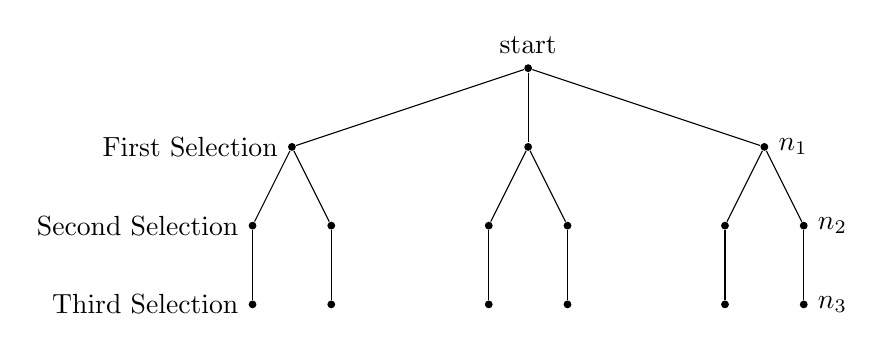
\begin{tikzpicture}
            [point/.style = {circle, fill, inner sep = 1pt}]
            \node[point] (1a) [label=above:start] at (6.5, 3) {};
            \node[point] (2a) [label=left:\text{First Selection}] at (3.5, 2) {};
            \node[point] (2b) at (6.5, 2) {};
            \node[point] (2c) [label=right:$n_1$] at (9.5, 2) {};
            \node[point] (3a) [label=left:\text{Second Selection}] at (3, 1) {};
            \node[point] (3b) at (4, 1) {};
            \node[point] (3c) at (6, 1) {};
            \node[point] (3d) at (7, 1) {};
            \node[point] (3e) at (9, 1) {};
            \node[point] (3f) [label=right:$n_2$] at (10, 1) {};
            \node[point] (4a) [label=left:\text{Third Selection}] at (3, 0) {};
            \node[point] (4b) at (4, 0) {};
            \node[point] (4c) at (6, 0) {};
            \node[point] (4d) at (7, 0) {};
            \node[point] (4e) at (9, 0) {};
            \node[point] (4f) [label=right:$n_3$] at (10, 0) {};
            \draw (1a) -- (2a);
            \draw (1a) -- (2b);
            \draw (1a) -- (2c);
            \draw (2a) -- (3a);
            \draw (2a) -- (3b);
            \draw (2b) -- (3c);
            \draw (2b) -- (3d);
            \draw (2c) -- (3e);
            \draw (2c) -- (3f);
            \draw (3a) -- (4a);
            \draw (3b) -- (4b);
            \draw (3c) -- (4c);
            \draw (3d) -- (4d);
            \draw (3e) -- (4e);
            \draw (3f) -- (4f);
        \end{tikzpicture}
    \end{center}
\end{ln-fig}
Say we are looking for the number of ordered sequences produced from sampling from a three-card deck. Then, we will once again have 3 possibilities for the first card, 2 for the second card, and 1 for the third card (provided it's the last card chosen). \\
In the above figure, each leaf node is a termination of the sampling process: a possibility. Therefore, we just count the number of leaf nodes that exist in this tree: in this case:
\[n_1 \times n_2 \times n_3 = 3 \times 2 \times 1 = 6\]

\subsection{Counting Sets}
Sets are slightly different stories from sequences, since there is no order in set. \\
Put in a deck drawing context as discussed in prior subsection, we would then be counting the number of distinct hands: where hands do not all have same members (cards). \\
To count the distinct subsets of a set $S$ (in this case our deck) with $5$ cards, we can let each sequence get placed into some bin corresponding to the set of 5 elements in the sequence. Each bin must contain $5!$ ways of ordering the $5$ elements in the set. \\
This means we just have to find the number of bins (distinct sets), which is essentially dividing the number of ordered sequences with $5!$ for this context:
\[\frac{52!}{(52 - 5)!5!}\]
This quantity, $\frac{n!}{(n - k)!k!}$, stands for the number of $k$-element subsets from an n-element set $S$, the result of our counting. The alternative but more popular expression of this is $\binom{n}{k}$:
\begin{ln-theorem}{Second Rule of Counting}{}
    Assume an object is made by a succession of choices, and the order in which the choices are made does not matter. \\
    Let $A$ be the set of ordered objects, $B$ the set of unordered objects. If there exists an m-to-1 function $f: A \rightarrow B$, then we can count the number of ordered objects and divide by $m$ to obtain the number of unordered objects.
\end{ln-theorem}
So in the hand-counting context of this subsection, we had a $5!$-to-$1$ function from set of all ordered sequences to set of all distinct hands (which are the unordered sequences we count for).

\section{Sampling with Replacement}
What are the mathematical properties of sampling with replacement? \\
Since no elements are removed from $S$, the number of possible choices across each selection will be constant, provided that the numebr of elements in $S$ is always constant and does not decrease. \\
And, since we have $n$ choices in each trial, across $k$ selections in the process of creating a $k$-length sequence, 
\[n_1 = n_2 = \cdots = n_k = n\]
Therefore, the total number of possible ordered $k$-length sequences from an $n$-element set $S$ under sample with replacement is $n^k$.

\subsection{Here is an Example}
We may visit coin tosses first. The total possible outcomes of tossing a coin $k=3$ times can be portrayed by the following tree:
\begin{ln-fig}{The Tree of Counting on Coins}{}
    \begin{center}
        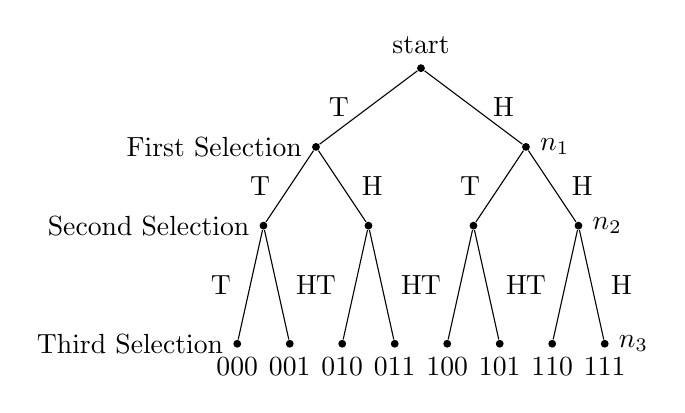
\begin{tikzpicture}
            [point/.style = {circle, fill, inner sep = 1pt}]
            \node[point] (1a) [label=above:start] at (7/3, 3) {};
            \node[point] (2a) [label=left:\text{First Selection}] at (3/3, 2) {};
            \node[point] (2b) [label=right:$n_1$] at (11/3, 2) {};
            \node[point] (3a) [label=left:\text{Second Selection}] at (1/3, 1) {};
            \node[point] (3b) at (5/3, 1) {};
            \node[point] (3c) at (9/3, 1) {};
            \node[point] (3d) [label=right:$n_2$] at (13/3, 1) {};
            \node[point] (4a) [label=left:\text{Third Selection}, label=below:$000$] at (0, -0.5) {};
            \node[point] (4b) [label=below:$001$] at (2/3, -0.5) {};
            \node[point] (4c) [label=below:$010$] at (4/3, -0.5) {};
            \node[point] (4d) [label=below:$011$] at (6/3, -0.5) {};
            \node[point] (4e) [label=below:$100$] at (8/3, -0.5) {};
            \node[point] (4f) [label=below:$101$] at (10/3, -0.5) {};
            \node[point] (4g) [label=below:$110$] at (12/3, -0.5) {};
            \node[point] (4h) [label=right:$n_3$, label=below:$111$] at (14/3, -0.5) {};
            \draw (1a) -- (2a) node [midway, label=left:T] {};
            \draw (1a) -- (2b) node [midway, label=right:H] {};
            \draw (2a) -- (3a) node [midway, label=left:T] {};
            \draw (2a) -- (3b) node [midway, label=right:H] {};
            \draw (2b) -- (3c) node [midway, label=left:T] {};
            \draw (2b) -- (3d) node [midway, label=right:H] {};
            \draw (3a) -- (4a) node [midway, label=left:T] {};
            \draw (3a) -- (4b) node [midway, label=right:H] {};
            \draw (3b) -- (4c) node [midway, label=left:T] {};
            \draw (3b) -- (4d) node [midway, label=right:H] {};
            \draw (3c) -- (4e) node [midway, label=left:T] {};
            \draw (3c) -- (4f) node [midway, label=right:H] {};
            \draw (3d) -- (4g) node [midway, label=left:T] {};
            \draw (3d) -- (4h) node [midway, label=right:H] {};
        \end{tikzpicture}
    \end{center}
\end{ln-fig}
In the above graph, each vertex corresponds to a possible result, where each bit stands for whether the toss resulted in a head (1) or a tail (0).

\subsection{But Sometimes, Order Doesn't Matter}
Suppose we would like to select 5 cards from a set of three cards $S = \{1, 2, 3\}$, where ordering doesn't matter. \\
In this context, Second Rule of Counting does not help, because we do not have a $m$-to-$1$ relationship between ordered sequences and distinct sets. We would need to apply a different perspective. Let us discuss below:

Let us first generalize back to the original setting. We have a set $S = \{1, 2, \cdots, n\}$ and would like to know the number of ways to choose multisets (sets with repetition) of size $k$. \\
Assume we have one bin for each element of $S$: providing $n$ bins in total. We then count the number of ways to fill these bins with $k$ elements, without minding the order of the bins themselves but just how many of the $k$ elements they each contain. \\
Each allocation to the bin can be written as a bit-string, where $1$ represents the change of bin and $0$ represents the existence of one element. \\
For example, provided $5$ bins and $5$ elements where the leftmost bin has $1$ element, the middle bin has $3$, adn the last has $1$, the representation is
\[01 10001 10\]
If there exists a space between the $1$s, it would imply that the bin contains no elements. \\
The length of our binary string, provided $n$ elements and $k$ bins, is $n + k - 1$. We now choose which $n$ locations should contain $0$s in this arbitrary zeros, or alternatively, which of the remaining $k-1$ containing $1$s. \\
A position corresponds to one specific value: once it is used, you may not reuse the position for another value and the position will be removed from the set of all possible options. The ordering also does not matter. \\
Therefore, we are essentially sampling $k$ locations from $k + n - 1$ without replacement where order does not matter, which provides the total number of multisets as:
\begin{ln-theorem}{Balls and Urns}{}
    Generally, the number of ways to place $n$ indistinguishable balls into $k$ distinguishable bins is:
    \[\binom{n + k - 1}{n} = \binom{n + k - 1}{k - 1}\]
\end{ln-theorem}
Let us also describe the intuition we have used in generating the balls and urns approach in producing a match between bitstrings and ball-urn allocations:
\begin{ln-theorem}{Zeroth Rule of Counting}{}
    If a set $A$ can be placed into a one-to-one correspondence with a set $B$ (in other words, find a bijection $f: A \rightarrow B$), then $|A| = |B|$.
\end{ln-theorem}
Upon which, let's attempt an elaboration on the knowledge of balls and urns:
\begin{ln-think}{Balls and Urns with No Empty Urns}{}
    Q: How many ways are there to put $n$ balls into $k$ urns such that there are no empty urns?
    \tcblower
    This is a variant of the balls and urns derivation, where instead of using $1$ to notate the boundary of bins, we use $01$ instead to ensure all bins on the left of some boundary receive at least one ball. Meanwhile, a character $0$ is put as the rightmost bit of the ball-urn representing bitstring. \\
    Now, how long is this bitstring, if we consider bits to be represented by $0$ and $01$ (instead of $1$)? \\
    We will realize that while $n - (k - 1)$ bits would be $0$, $k - 1$ bits would be $01$. Furthermore, we are only permitted $n - 1$ positions to freely choose on the insertion of $0$ (since $k - 1$ of $0$s are used in bin boundaries, and another 1 is put as the rightmost bit of the bitstring). \\
    Therefore, the number of ways balls and urns operate with no empty bins would be:
    \[\binom{n - 1}{k - 1}\]
\end{ln-think}

\section{Combinatorial Proofs}
In short, proofs on combinatorials. They are mostly identity proofs. Let us explore a few examples/categories from below sections:

\subsection{Binomial Theorem}
\begin{ln-theorem}{Binomial Theorem}{}
    \[\forall n \in \N, {(a + b)}^n = \sum_{k = 0}^n \binom{n}{k} a^k b^{n - k}\]
    \tcblower
    \textbf{Proof}: \\
    The LHS is a product of $n$ terms $(a + b)$. \\
    Let these factors be labeled sets $f_1, \dots, f_n$ for generality. \\
    For multiplying factors $f_1$, $f_2$, a total of $4$ two-term combinations is made via matching each term of $f_1$ to each term of $f_2$:
    \[f_1 \times f_2 = \{(a_{f_1}, a_{f_2}), (a_{f_1}, b_{f_2}), (b_{f_1}, a_{f_2}), (b_{f_1}, b_{f_2})\}\]
    \[(a + b)^2 = a^2 + ab + ba + b^2\]
    Every term in such polynomial is in some form $a^k b^{n - k}$. It would be reasonable to see how this term contributes to the over sums of polynomial. \\
    We produce terms $a^k b^{n - k}$ when $k$ copies of $a$ and $n$ copies of $b$ are multiplied, and there are $\binom{n}{k}$ ways to form such terms. \\
    Therefore, for each index $k$ possible (which spans from $0$ to $n$, standing for the number of $a$ apparent in the monomial), the sum of such monomials is the product of its value and number of such pairing:
    \[\binom{n}{k} a^k b^{n - k}\]
    Sum this product over all possible $k$, we will get the value of ${(a + b)}^n$, which is the sum of all possible monomials (products) achieved:
    \[\sum_{k = 0}^n \binom{n}{k} a^k b^{n - k}\]
\end{ln-theorem}

The Binomial Theorem would then contribute to an interesting identity. Let us set $a = 1$, $b = -1$ in binomial theorem. Then:
\begin{align*}
    (-1 + 1)^n
    &= \sum_{k = 0}^n \binom{n}{k} {(-1)}^k {(1)}^{n - k} \\
    &= \sum_{k = 0}^n \binom{n}{k} {(-1)}^k = 0
\end{align*}
Huh, what! Did you just use binomial theorem to prove that $-1 + 1 = 0$ to the $n^{th}$ power is still $0$? \\
Yeah, we did. But the last line of the proof, which is the combinatorial identity we have produced, is arugably more valuable.

\subsection{Combinatorial Identities}
Here are two interesting combinatorial identities to capitalize off in several proofs.

For now, let's talk about the first of two:
\begin{ln-theorem}{Hockey-Stick Identity}{}
    The Hockey-Stick Identity states that:
    \[\binom{n}{k + 1} = \sum_{i = k}^{n - 1} \binom{i}{k}\]
    \tcblower
    \textbf{Combinatorial Proof}:
    The LHS of this identity is the number of ways to choose a $(k + 1)$-length subset from an $n$-element set $S$. \\
    For generality, let us denote $S$ such that:
    \[S = \{S_1, \cdots, S_n\},\ \ S_1 < \cdots < S_n\]
    Make the following observation on how we can produce subsets:
    \begin{bindenum}
        \item If we let the lowest-value element of the subset to be $S_1$, then we will have $k$ elements to choose from the rest of $n - 1$ elements from $S$. Therefore, it contributes $\binom{n - 1}{k}$ to the total number of combinations.
        \item If we let the lowest-value element of the subset to be $S_i$, then we will have $k$ elements to choose from the rest of $n - i$ elements from $S$ (because $i$ elements of $S$ are smaller than or equal to the smallest element of subset). Therefore, it contributes $\binom{n - i}{k}$ to the total number of combinations.
    \end{bindenum}
    This sum will continue until we let the lowest-value element of subset to be $S_{n - k}$, where we would be left with $n - (n - k) = k$ elements to choose from: the bare minimum. \\
    Totaling all above contribution leads to the Hockey-Stick Identity.
\end{ln-theorem}

The second identity I'd like to introduce to you is:
\begin{ln-theorem}{Sum of combinations from $n$ items}{}
    \[\sum_{k = 0}^n \binom{n}{k} = 2^n\]
    \tcblower
    This identity can be proved via setting $a = 1$, $b = 1$ from the binomial theorem:
    \begin{align*}
        2^n &= (1 + 1)^n \\
        &= \sum_{k = 0}^n \binom{n}{k} {1}^k {1}^{n - k} \\
        &= \sum_{k = 0}^n \binom{n}{k} {1}^k = \sum_{k = 0}^n \binom{n}{k}
    \end{align*}
    To discuss this via combinatorial proof (which is via interpretation of both sides of equation), suppose we have a set $S$ with $n$ distinct elements. \\
    The LHS of this identity counts the number of ways of choosing an $i$-lengthed subset. \\
    The RHS, meanwhile, counts the total number of possible subsets (see the Chapter for Set Theory in this document). \\
    Therefore, the LHS and RHS of this identity indeed denote the same value!
\end{ln-theorem}


\subsection{Permutation and Derangements}
Assume that we collect the namecard of $n$ people, and redistribute them into the $n$ people. On average, how many people recieve their own namecard?

Let us look at this in a combinatorics perspective. \\
Label the namecards as $1, 2, \cdots, n$ and let $\pi_i$ denote the namecard that is returned to the $i^{th}$ student. \\
Then, the vector $\vec{\pi} = \begin{bmatrix} \pi_1 & \cdots & \pi_n \end{bmatrix}^T$: a permutation of the set $\{1, \cdots, n\}$. There are then $n!$ distinct permutations of $\{1, \dots, n\}$ since it is not a multiset. \\
In this setting, the situation at which a person receives his own namecard is when $\pi_i = i$. \\
Therefore, the number of people who receive their own namecard is the amount of index at which $\pi_i = i$. These points are called ``fixed points''.

A permutation with no fixed points is called a \textbf{derangement}. \\
There is a formula for the number of derangements provided a set of $n$ distinct elements:
\begin{ln-theorem}{Number of Derangements}{}
    \textbf{Theorem}: For an arbitrary positive integer $n \geq 3$, the number $D_n$ of derangements of $\{1, \dots, n\}$ satisfies:
    \[D_n = (n - 1)(D_{n - 1} + D_{n - 2})\]
    \tcblower
    \textbf{Proof}: \\
    In a derangement $(\pi_1, \cdots, \pi_n)$, suppose $\pi_n = j \in \{1, \cdots, n - 1\}$. Then, there are $n - 1$ choices for $j$. We also know that $j \neq n$ because this would then not produce a derangement. \\
    Now, if $\pi_j = n$, then we recognize that $j$ and $n$ get swapped, and the number of possible derangements with the remaining $n - 2$ numbers is $D_{n - 2}$. \\
    Or, if $\pi_j \neq n$, then $n$ satisfies the same constraint as $j$ (in not being able to be the value $j$). Therefore, we have $n - 1$ values left to form derangements with, which provides $D_{n - 1}$ possibilities. \\
    This completes the derivation of the above formula.
\end{ln-theorem}
Notably, with the boundary conditions $D_1 = 0$ and $D_2 = 1$, we can then determine $D_n$ computationally via recursion and rather efficiently with the use of memoization. \\
The derivation is not shown here, but the recursion would then yield that:
\[D_n = n! \sum_{k = 0}^n \frac{{(-1)}^k}{k!}\]

\section{The Principle of Inclusion-Exclusion}
Overcounting is a big problem in combinatorics, but here is a technique to prevent most of such situations. \\
Let $A_1$ and $A_2$ be two subsets of the same finite set $A$ and we want to count the number of elements in $A_1 \cup A_2$. \\
If $A_1$ and $A_2$ are disjoint, it is very lucky:
\[|A_1 \cup A_2| = |A_1| + |A_2|\]
If $A_1$ and $A_2$ are not disjoint, however, then we need to subtract the number of elements from their intersections:
\[|A_1 \cup A_2| = |A_1| + |A_2| - |A_1 \cap A_2|\]
This brings us to the generalization of this logic over an arbitrary number of subsets:
\begin{ln-theorem}{Principle of Inclusion-Exclusion}{}
    \textbf{Theorem}: Let $A_1, \cdots, A_n$ be arbitrary subsets of the same finite set $A$:
    \[|A_1 \cup \cdots \cup A_n| = \sum_{k = 1}^n {(-1)}^{k - 1} \sum_{S \subseteq \{1, \cdots, n\}:|S| = k} |\cap_{i \in S}A_i|\]
    \tcblower
    \textbf{Proof}: \\
    Note that if $a$, an element, is not included by the union of all subsets of $A$ considered in this scenario, then it is not possible for $a$ to be counted anyways. \\
    For $a$ to be counted, it must belong to some subset $A_i$, such that $i \in \{1, \dots, m\}$. \\
    For the sake of clarifying the proof, define an index set $M \subseteq \{1, \dots, n\}$ as:
    \[M = \{i \in \{1, \dots, n\}:\ a \in A_i\}\]
    applying the prior logic, $a \in A_i$ iff $i \in M$. Here, if the subset $S$ we find is not contained by $M$, then $a \notin \cap_{i \in S}A_i$. \\
    Therefore, for $a$ to be counted, $a \in \cap_{i \in S}A_i$ for any non-empty subset $S \subseteq M$. \\
    The number of subsets that have counted $a$ on RHS is thus:
    \[\sum_{k = 1}^n {(-1)}^{k - 1} \sum_{S \subseteq \{1, \cdots, n\}:|S| = k} 1 = \sum_{k = 0}^m \binom{m}{k} {(-1)}^{k - 1} = 1\]
\end{ln-theorem}
On the perspective of some venn diagram of events, inclusion-exclusion principle serves to calculate the net area of venn diagram by repeating the process of subtracting overlapped regions and adding back over-subtracted regions. \\
It is notable that, however, inclusion-exclusion used in probabilistic contexts provide diminishing marginal utility due to computational cost, and usually perform a good enough job at the third iteration of adding/subtracting areas.

And applying this to the derangement problem:
\begin{ln-quest}{Count Derangements}{}
    Let $A_i$ denote the set of all permutations with $i$ being a fixed point. \\
    The number of permutations with at least one fixed point is $|A_1 \cup \cdots \cup A_n|$. Therefore,
    \[D_n = n! - |A_1 \cup \cdots \cup A_n|\]
    Meanwhile, the cardinality of $A_i$ would be $(n - 1)!$ because it just has to permute $n - 1$ other elements in an arbitrary way. \\
    The intersection of $A_i$ and $A_j$ would thus need to permute $n - 2$ arbitrary elements, and has cardinality $(n - 2)!$. \\
    Let us follow the clue: for a subset $S \in \{1, \cdots, n\}$ such that $|S| = k$,
    \[|\cap_{i \in S} A_i| = (n - k)!\]
    The rest of algebra follows:
    \begin{align*}
        |A_1 \cup \cdots \cup A_n|
        &= \sum_{k = 1}^n {(-1)}^{k - 1} \binom{n}{k} (n - k)! \\
        &= \sum_{k = 1}^n {(-1)}^{k - 1} \frac{n!}{k!} \\
        &= n! \sum_{k = 1}^n {(-1)}^{k - 1} \frac{1}{k!} \\
        D_n
        &= n! - |A_1 \cup \cdots \cup A_n| \\
        &= n! (1 - \sum_{k = 1}^n {(-1)}^{k - 1} \frac{1}{k!}) \\
        &= n! \sum_{k = 1}^n \frac{{(-1)}^{k}}{k!}
    \end{align*}
\end{ln-quest}

\section{Personal Regards on this Topic}
The biggest takeaways from this chapter would be the ability to answer the following questions:
\begin{bindenum}
    \item In the counting problem I work at, does order matter?
    \item In the counting problem I work at, is sampling with or without replacement?
    \item How do I perform combinatorial proofs by creating stories (interpretation of combinatorial expression) for both sides of the equations?
    \item How do I setup counting problems and see what object do I exactly need to count?
\end{bindenum}
And combinatorial identities can prove useful if you bring them along on cheat sheets; as you see, combinatorial arguments of this chapter have hugely relied on the power of many combinatorial identities.
